\documentclass[portrait,color=UCLburgundy,margin=2cm]{uclposter}

\newcommand{\boldf}{\bm{f}}
\newcommand{\boldmu}{\bm{\mu}}
\newcommand{\boldalpha}{\bm{\alpha}}
\newcommand{\boldr}{\bm{r}}
\newcommand{\boldt}{\bm{t}}
\newcommand{\boldg}{\bm{g}}
\newcommand{\boldtheta}{\bm{\theta}}

% Warping operators
\newcommand{\MPWarp}{\tilde{\mathcal{W}}}
\newcommand{\Warp}{\mathcal{W}}

% Others
\newcommand{\etal}{\textit{et al.}~}
\newcommand{\ie}{i.e., }
\newcommand{\eg}{e.g., }

\usepackage{bm}
\usepackage{algorithm}
\usepackage{algorithmic}
\usepackage{caption}

\usepackage[acronym]{glossaries}
\newacronym{mu map}{mu map}{Attenuation Map}
\newacronym{TOF}{TOF}{Time-Of-Flight}
\newacronym{NAC}{NAC}{Non-Attenuation-Corrected}
\newacronym{RCM}{RCM}{Respiratory Correspondence Model}
\newacronym{MAPE}{MAPE}{Mean Absolute Percentage Error}
\newacronym{COM}{COM}{Centre Of Mass}
\newacronym{SIRF}{SIRF}{Synergistic Image Reconstruction Framework}
\newacronym{AP}{AP}{Anterior-Posterior}
\newacronym{IS}{IS}{Inferior-Superior}

\usepackage[style=ieee,maxbibnames=1,minbibnames=1,maxcitenames=1,mincitenames=1,backend=biber,defernumbers=false]{biblatex}
\addbibresource{./Biblio.bib}

\usepackage{fontspec}
\setmainfont[Ligatures=TeX]{LexendDeca-Regular.ttf}

\begin{document}

\title{Impact of Time-of-Flight on Respiratory Motion\newline Modelling using Non-Attenuation-Corrected PET}

\author[1,2 *]{Alexander C. Whitehead}
\author[1]{Elise C. Emond}
\author[3]{Nikos Efthimiou}
\author[1,2]{Adeyemi Akintonde}
\author[4]{Scott Wollenweber}
\author[4]{\newline Charles Stearns}
\author[1]{Brian F. Hutton}
\author[2]{Jamie R. McClelland}
\author[1]{Kris Thielemans}

\affil[1]{INM, University College London, UK}
\affil[2]{CMIC, University College London, UK\newline}
\affil[3]{PET Research Centre, University of Hull, UK}
\affil[4]{MICT Engineering, GE Healthcare, USA\newline}
\affil[*]{alexander.whitehead.18@ucl.ac.uk}

\maketitle

\vspace{-1.0cm}

\begin{multicols}{2}
\normalsize

\section*{Introduction}
\begin{highlightbox}[UCLlightgreen]
    \begin{itemize}
        \item Respiratory motion causes artefacts and loss of resolution in PET. Surrogate driven motion models attempt to overcome these deficiencies by relating the motion in the data to a surrogate signals \cite{McClelland2017}.
        \item If images are reconstructed using a static \gls{mu map}, then artefacts caused by the misalignment between the activity distribution and the \gls{mu map} would hamper image registration.
        \item The aim of this work is to investigate whether \gls{TOF} information can sufficiently increase the contrast and lower the noise of \gls{NAC} images to facilitate the fitting of accurate motion models.
    \end{itemize}
\end{highlightbox}

\section*{Methods}
\begin{itemize}

    \vspace{1.0cm}
    
    \subsection*{\underline{\textbf{Simulation}}}
    
    \vspace{-1.0cm}
    
    \item XCAT was used to generate volumes, the field of view included the lungs and diaphragm and a 40mm diameter spherical lesion placed in the right lung.
    \item  Acquisitions were simulated using STIR \cite{Efthimiou2018} through SIRF using the geometry of a GE Discovery 710 and a \gls{TOF} resolution of 375ps, similar to the GE Signa.
    \item Attenuation was included in the simulation.
    \item  Acquisitions were simulated as if they had been gated into 6 bins over an acquisition of 120s (30 million true counts).
    
    \subsection*{\underline{\textbf{Reconstruction}}}
    \item Data were reconstructed without attenuation correction using OSEM with 24 subsets and 2 full iterations and were post filtered using a Gaussian blurring with a size of 6.4mm.
    
    \subsection*{\underline{\textbf{Motion Estimation}}}
    \item A \gls{RCM} parametrises motion fields in terms of a surrogate signals representing the breathing motion.
    \item A generalized framework unifying image registration and respiratory motion models, NiftyRegResp, \cite{McClelland2017} was used to fit a direct correspondence motion model with B-spline motion fields. The B-spline coefficients at time \resizebox*{!}{10mm}{$t$} are expressed as a linear combination of the 2 components of the surrogate, \resizebox*{!}{15mm}{$s_{1,t}$} and \resizebox*{!}{15mm}{$s_{2,t}$}, the \gls{AP} and \gls{IS} motion derived from the input to XCAT:
\end{itemize}

\vspace{-2.0cm}
    
\begin{center}
    \resizebox*{1.0\hsize}{!}{$\forall t \in [[1,n_t]], \quad\alpha_{k,t} := R_{1,k} s_{1,t} + R_{2,k} s_{2,t} + R_{3,k}$}
\end{center}

\vspace{-1.0cm}
    
\indent where \resizebox*{!}{20mm}{$\quad{\alpha}_{k,t} = \left\{\alpha^X_{k,t}, \alpha^Y_{k,t}, \alpha^Z_{k,t}\right\}$} is a vector of B-spline coefficients for node \resizebox*{!}{10mm}{$k$} at time point \resizebox*{!}{10mm}{$t$}, and \resizebox*{!}{15mm}{$R_{i,k}$} are the associated model parameters.
    
\begin{highlightbox}[UCLlightgreen]
    \subsection*{\underline{\textbf{Evaluation}}}
    3 \gls{RCM}s were compared, calculated from the XCAT volumes (best case scenario), non-\gls{TOF} \gls{NAC} and \gls{TOF} \gls{NAC} reconstructions. These were used to warp a reference volume. The warped volumes were then compared to the original XCAT volumes.
\end{highlightbox}

\end{multicols}

\vspace{-2.0cm}

\rule{1\hsize}{0.1cm}

\vspace{-2.0cm}

\section*{Results}

\begin{figure*}[h!]
  \centering
  
  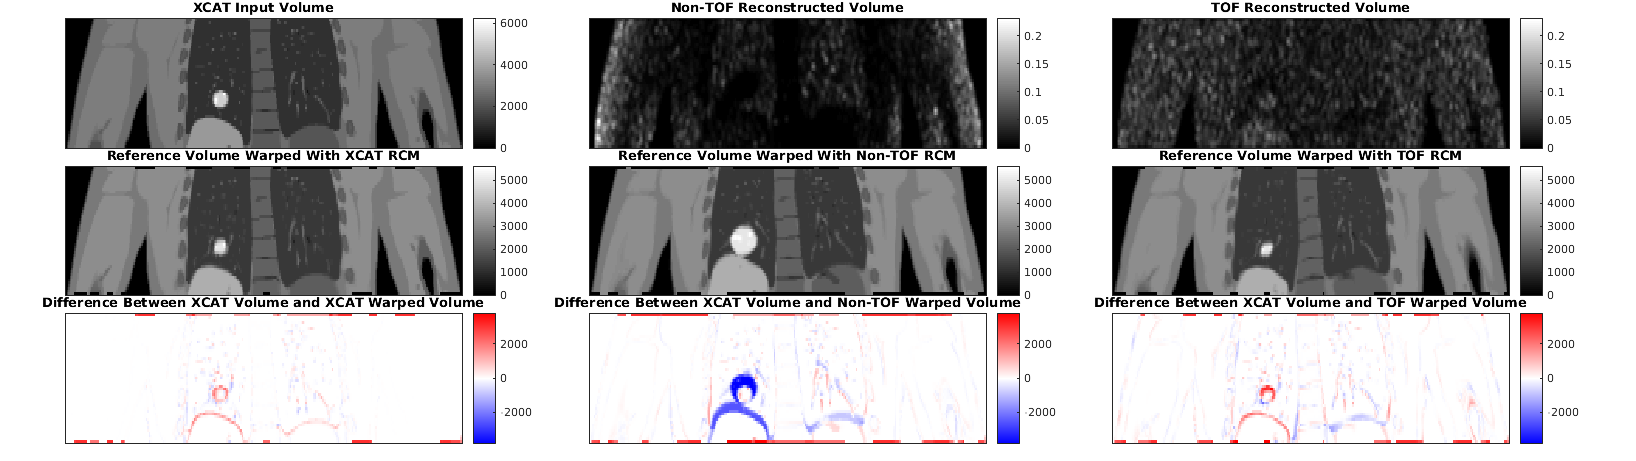
\includegraphics[width=1\linewidth]{output.png}
  
  \begin{highlightbox}[UCLlightblue]
    \captionsetup{singlelinecheck=false, justification=centering}
    \caption{All volumes correspond to end inhalation. First row from left to right: XCAT PET, NAC non-TOF and NAC TOF reconstructed data. Second row: RCM applied to reference position XCAT data with RCM derived from XCAT PET data (left), NAC non-TOF (middle) and NAC TOF (right) volumes. The third row: The difference between the estimated volumes from the second row with the XCAT end inhalation volume.}
  \end{highlightbox}
  
  \label{fig:output}
\end{figure*}

\vspace{-0.25cm}

\begin{multicols}{2}

\begin{table}[H]
  \centering
  
  \begin{highlightbox}[UCLlightblue]
    \captionsetup{singlelinecheck=false, justification=centering}
    \caption{Comparison of the \gls{MAPE} between each ground truth volume and its corresponding volume estimated by warping a reference volume using, in turn, the XCAT, the \gls{NAC} non-\gls{TOF} and the \gls{NAC} \gls{TOF} based \gls{RCM}.}
  \end{highlightbox}
  
  \vspace{0.5cm}
  
  \resizebox*{0.6\linewidth}{!}
  {
    \begin{tabular}{||c|ccc||}
      \hline
        \textbf{\gls{MAPE}} & \textbf{XCAT} & \textbf{non-\gls{TOF}} & \textbf{\gls{TOF}} \\
      \hline
        \textbf{1} & 1.95 & 8.35 & 4.18 \\
        \textbf{2} & 1.59 & 1.61 & 1.84 \\
        \textbf{3} & 2.06 & 9.91 & 5.23 \\
        \textbf{4} & 1.97 & 6.15 & 3.68 \\
        \textbf{5} & 1.65 & 4.45 & 2.52 \\
        \textbf{6} & 1.95 & 8.35 & 4.18 \\
      \hline
        \textbf{Mean} & 1.86 & 6.47 & 3.60 \\
      \hline
    \end{tabular}
  }
  \label{tab:MAPE}
\end{table}

\begin{figure}[H]
  \centering
  
  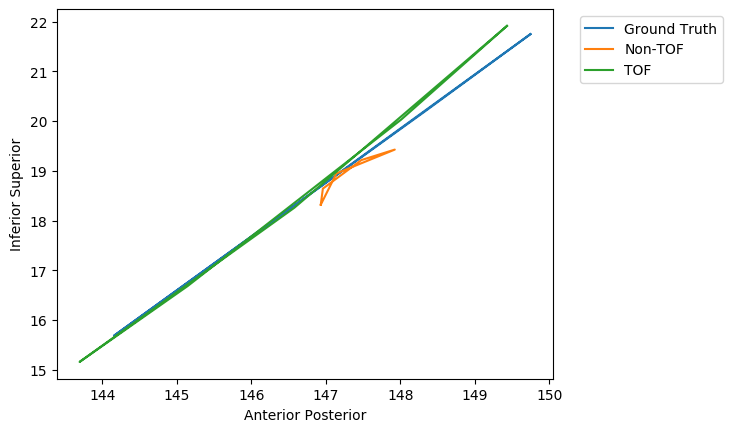
\includegraphics[width=0.8\linewidth]{TOF.png}
  
  \begin{highlightbox}[UCLlightblue]
    \captionsetup{singlelinecheck=false, justification=centering}
    \caption{The path of the \gls{COM} of the lesion. Different curves denote \gls{COM} for ground truth, XCAT, \gls{NAC} non-\gls{TOF} and \gls{NAC} \gls{TOF} based \gls{RCM} estimated data}
  \end{highlightbox}
  
  \label{fig:com_graph}
\end{figure}

\end{multicols}

\vspace{-2.0cm}

\rule{1\hsize}{0.1cm}

\vspace{-1.0cm}

\begin{multicols}{2}
\normalsize

\section*{Conclusion}
\begin{itemize}
    \item NAC nonTOF images were not suitable to provide an estimate of the motion. However, when using TOF, the obtained motion models were able to recover the motion of the lesion and other structures.
    \item Future research will investigate the robustness of the motion model estimation to different noise levels, acquisition duration and size of lesion.
\end{itemize}

\AtNextBibliography{\small}
\printbibliography

\small
\section*{Acknowledgements}
This research is supported by GE Healthcare, the NIHR UCLH Biomedical Research Centre and the EPSRC funded UCL Centre for Doctoral Training in Medical Imaging (EP/L016478/1). Elise C. Emond is supported by GlaxoSmithKline (BIDS3000030921). Jamie R. McClelland is supported by a Cancer Research UK Centres Network Accelerator Award Grant (A21993) to the ART-NET consortium and a CRUK Multi-disciplinary grant (CRC 521).

\end{multicols}

\end{document}
